\documentclass{article}
\usepackage{graphicx} % Required for inserting images

\usepackage[margin=1in]{geometry}

\usepackage{amsmath}
\usepackage{amsthm}
\usepackage{amsfonts}
\usepackage{amssymb}

%% Local macros
\renewcommand{\le}{\leqslant} 
\renewcommand{\ge}{\geqslant} 
\renewcommand{\leq}{\leqslant} 
\renewcommand{\geq}{\geqslant} 
\newcommand{\eset}{\varnothing}
\newcommand{\ra}{\rangle}
\newcommand{\la}{\langle} 
\newcommand{\wt}{\widetilde}
\newcommand{\pms}{\{-1,1\}}
\newcommand{\ind}{\mathbf{1}}
\providecommand{\1}{\mathbb{1}} 
\newcommand{\eps}{\varepsilon}
\newcommand{\To}{\longrightarrow}
\newcommand{\norm}[1]{\left\Vert#1\right\Vert}
\newcommand{\abs}[1]{\left\vert#1\right\vert}
\newcommand{\set}[1]{\left\{#1\right\}}
\newcommand{\goesto}{\longrightarrow}
\newcommand{\Real}{\mathbb{R}}
\newcommand{\Complex}{\mathbb{C}}
\newcommand{\ie}{\emph{i.e.,}}
\newcommand{\as}{\emph{a.e.}}
\newcommand{\eg}{\emph{e.g.,}}
\renewcommand{\iff}{\Leftrightarrow} 
\newcommand{\equald}{\stackrel{\mathrm{d}}{=}}
\newcommand{\probc}{\stackrel{\mathrm{P}}{\longrightarrow}}
\newcommand{\weakc}{\stackrel{\mathrm{w}}{\longrightarrow}}
\newcommand{\fpar}[2]{\frac{\partial #1}{\partial #2}}
\newcommand{\spar}[2]{\frac{\partial^2 #1}{\partial #2^2}}
\newcommand{\mpar}[3]{\frac{\partial^2 #1}{\partial #2 \partial #3}}  
\def\qed{ \hfill $\blacksquare$}  
\newcommand{\cbs}{\mathcal{B}_\star}
\newcommand{\obs}{\overline{\mathcal{B}}_\star}
%% End Local macros
%%%%%%%%%%%%%%%%%%%%%%%%%%%%%%%%%%%%%%%%%%%
%%%%%%%%%%%%%%%%%%%%%%%%%%%%%%%%%%%%%%%%%%%
%% Greek symbols
\let\ga=\alpha \let\gb=\beta \let\gc=\gamma \let\gd=\delta \let\gee=\epsilon
\let\gf=\varphi \let\gh=\eta \let\gi=\iota  \let\gk=\kappa \let\gl=\lambda \let\gm=\mu    \let\gn=\nu \let\go=\omega \let\gp=\pi \let\gr=\rho \let\gs=\sigma \let\gt=\tau \let\gth=\vartheta
\let\gx=\chi \let\gy=\upsilon \let\gz=\zeta
\let\gC=\Gamma \let\gD=\Delta \let\gF=\Phi \let\gL=\Lambda \let\gTh=\Theta
\let\gO=\Omega   \let\gP=\Pi    \let\gPs=\Psi  \let\gS=\Sigma \let\gU=\Upsilon \let\gX=\Chi
\let\gY=\Upsilon                                
%% End Greek Symbols
%%%%%%%%%%%%%%%%%%%%%%%%%%%%%%%%%%%%%%%%%%%
%%%%%%%%%%%%%%%%%%%%%%%%%%%%%%%%%%%%%%%%%%%
%% MathCal symbols
%\newcommand{\mc}[1]{\mathcal{#1}}
\newcommand{\cA}{\mathcal{A}}\newcommand{\cB}{\mathcal{B}}\newcommand{\cC}{\mathcal{C}}
\newcommand{\cD}{\mathcal{D}}\newcommand{\cE}{\mathcal{E}}\newcommand{\cF}{\mathcal{F}}
\newcommand{\cG}{\mathcal{G}}\newcommand{\cH}{\mathcal{H}}\newcommand{\cI}{\mathcal{I}}
\newcommand{\cJ}{\mathcal{J}}\newcommand{\cK}{\mathcal{K}}\newcommand{\cL}{\mathcal{L}}
\newcommand{\cM}{\mathcal{M}}\newcommand{\cN}{\mathcal{N}}\newcommand{\cO}{\mathcal{O}}
\newcommand{\cP}{\mathcal{P}}\newcommand{\cQ}{\mathcal{Q}}\newcommand{\cR}{\mathcal{R}}
\newcommand{\cS}{\mathcal{S}}\newcommand{\cT}{\mathcal{T}}\newcommand{\cU}{\mathcal{U}}
\newcommand{\cV}{\mathcal{V}}\newcommand{\cW}{\mathcal{W}}\newcommand{\cX}{\mathcal{X}}
\newcommand{\cY}{\mathcal{Y}}\newcommand{\cZ}{\mathcal{Z}}  
%% End MathCal symbols
%%%%%%%%%%%%%%%%%%%%%%%%%%%%%%%%%%%%%%%%%%%
%%%%%%%%%%%%%%%%%%%%%%%%%%%%%%%%%%%%%%%%%%%
%% Math Boldface Symbols
\newcommand{\vzero}{\mathbf{0}}\newcommand{\vone}{\mathbf{1}}\newcommand{\vtwo}{\mathbf{2}}
\newcommand{\vthree}{\mathbf{3}}\newcommand{\vfour}{\mathbf{4}}\newcommand{\vfive}{\mathbf{5}}
\newcommand{\vsix}{\mathbf{6}}\newcommand{\vseven}{\mathbf{7}}\newcommand{\veight}{\mathbf{8}}
\newcommand{\vnine}{\mathbf{9}}\newcommand{\vA}{\mathbf{A}}\newcommand{\vB}{\mathbf{B}}
\newcommand{\vC}{\mathbf{C}}\newcommand{\vD}{\mathbf{D}}\newcommand{\vE}{\mathbf{E}}
\newcommand{\vF}{\mathbf{F}}\newcommand{\vG}{\mathbf{G}}\newcommand{\vH}{\mathbf{H}}
\newcommand{\vI}{\mathbf{I}}\newcommand{\vJ}{\mathbf{J}}\newcommand{\vK}{\mathbf{K}}
\newcommand{\vL}{\mathbf{L}}\newcommand{\vM}{\mathbf{M}}\newcommand{\vN}{\mathbf{N}}
\newcommand{\vO}{\mathbf{O}}\newcommand{\vP}{\mathbf{P}}\newcommand{\vQ}{\mathbf{Q}}
\newcommand{\vR}{\mathbf{R}}\newcommand{\vS}{\mathbf{S}}\newcommand{\vT}{\mathbf{T}}
\newcommand{\vU}{\mathbf{U}}\newcommand{\vV}{\mathbf{V}}\newcommand{\vW}{\mathbf{W}}
\newcommand{\vX}{\mathbf{X}}\newcommand{\vY}{\mathbf{Y}}\newcommand{\vZ}{\mathbf{Z}}
\newcommand{\va}{\mathbf{a}}\newcommand{\vb}{\mathbf{b}}\newcommand{\vc}{\mathbf{c}}
\newcommand{\vd}{\mathbf{d}}\newcommand{\ve}{\mathbf{e}}\newcommand{\vf}{\mathbf{f}}
\newcommand{\vg}{\mathbf{g}}\newcommand{\vh}{\mathbf{h}}\newcommand{\vi}{\mathbf{i}}
\newcommand{\vj}{\mathbf{j}}\newcommand{\vk}{\mathbf{k}}\newcommand{\vl}{\mathbf{l}}
\newcommand{\vm}{\mathbf{m}}\newcommand{\vn}{\mathbf{n}}\newcommand{\vo}{\mathbf{o}}
\newcommand{\vp}{\mathbf{p}}\newcommand{\vq}{\mathbf{q}}\newcommand{\vr}{\mathbf{r}}
%\newcommand{\vs}{\mathbf{s}}\newcommand{\vt}{\mathbf{t}}\newcommand{\vu}{\mathbf{u}}
%\newcommand{\vv}{\mathbf{v}}\newcommand{\vw}{\mathbf{w}}\newcommand{\vx}{\mathbf{x}}
\newcommand{\vy}{\mathbf{y}}\newcommand{\vz}{\mathbf{z}} 
%% End Math Boldface Symbols
%%%%%%%%%%%%%%%%%%%%%%%%%%%%%%%%%%%%%%%%%%%
%%%%%%%%%%%%%%%%%%%%%%%%%%%%%%%%%%%%%%%%%%%  
%% Math Bold Symbols commands  
\newcommand{\mv}[1]{\boldsymbol{#1}}\newcommand{\mvinfty}{\boldsymbol{\infty}}\newcommand{\mvzero}{\boldsymbol{0}}
\newcommand{\mvone}{\boldsymbol{1}}\newcommand{\mvtwo}{\boldsymbol{2}}\newcommand{\mvthree}{\boldsymbol{3}}
\newcommand{\mvfour}{\boldsymbol{4}}\newcommand{\mvfive}{\boldsymbol{5}}\newcommand{\mvsix}{\boldsymbol{6}}
\newcommand{\mvseven}{\boldsymbol{7}}\newcommand{\mveight}{\boldsymbol{8}}\newcommand{\mvnine}{\boldsymbol{9}}
\newcommand{\mvA}{\boldsymbol{A}}\newcommand{\mvB}{\boldsymbol{B}}\newcommand{\mvC}{\boldsymbol{C}}
\newcommand{\mvD}{\boldsymbol{D}}\newcommand{\mvE}{\boldsymbol{E}}\newcommand{\mvF}{\boldsymbol{F}}
\newcommand{\mvG}{\boldsymbol{G}}\newcommand{\mvH}{\boldsymbol{H}}\newcommand{\mvI}{\boldsymbol{I}}
\newcommand{\mvJ}{\boldsymbol{J}}\newcommand{\mvK}{\boldsymbol{K}}\newcommand{\mvL}{\boldsymbol{L}}
\newcommand{\mvM}{\boldsymbol{M}}\newcommand{\mvN}{\boldsymbol{N}}\newcommand{\mvO}{\boldsymbol{O}}
\newcommand{\mvP}{\boldsymbol{P}}\newcommand{\mvQ}{\boldsymbol{Q}}\newcommand{\mvR}{\boldsymbol{R}}
\newcommand{\mvS}{\boldsymbol{S}}\newcommand{\mvT}{\boldsymbol{T}}\newcommand{\mvU}{\boldsymbol{U}}
\newcommand{\mvV}{\boldsymbol{V}}\newcommand{\mvW}{\boldsymbol{W}}\newcommand{\mvX}{\boldsymbol{X}}
\newcommand{\mvY}{\boldsymbol{Y}}\newcommand{\mvZ}{\boldsymbol{Z}}\newcommand{\mva}{\boldsymbol{a}}
\newcommand{\mvb}{\boldsymbol{b}}\newcommand{\mvc}{\boldsymbol{c}}\newcommand{\mvd}{\boldsymbol{d}}
\newcommand{\mve}{\boldsymbol{e}}\newcommand{\mvf}{\boldsymbol{f}}\newcommand{\mvg}{\boldsymbol{g}}
\newcommand{\mvh}{\boldsymbol{h}}\newcommand{\mvi}{\boldsymbol{i}}\newcommand{\mvj}{\boldsymbol{j}}
\newcommand{\mvk}{\boldsymbol{k}}\newcommand{\mvl}{\boldsymbol{l}}\newcommand{\mvm}{\boldsymbol{m}}
\newcommand{\mvn}{\boldsymbol{n}}\newcommand{\mvo}{\boldsymbol{o}}\newcommand{\mvp}{\boldsymbol{p}}
\newcommand{\mvq}{\boldsymbol{q}}\newcommand{\mvr}{\boldsymbol{r}}\newcommand{\mvs}{\boldsymbol{s}}
\newcommand{\mvt}{\boldsymbol{t}}\newcommand{\mvu}{\boldsymbol{u}}\newcommand{\mvv}{\boldsymbol{v}}
\newcommand{\mvw}{\boldsymbol{w}}\newcommand{\mvx}{\boldsymbol{x}}\newcommand{\mvy}{\boldsymbol{y}}
\newcommand{\mvz}{\boldsymbol{z}}
\newcommand{\mvga}{\boldsymbol{\alpha}}\newcommand{\mvgb}{\boldsymbol{\beta}}\newcommand{\mvgc}{\boldsymbol{\gamma}}
\newcommand{\mvgC}{\boldsymbol{\Gamma}}\newcommand{\mvgd}{\boldsymbol{\delta}}\newcommand{\mvgD}{\boldsymbol{\Delta}}
\newcommand{\mvgee}{\boldsymbol{\epsilon}}\newcommand{\mveps}{\boldsymbol{\eps}}\newcommand{\mvgf}{\boldsymbol{\varphi}}
\newcommand{\mvgF}{\boldsymbol{\Phi}}\newcommand{\mvgth}{\boldsymbol{\theta}}\newcommand{\mvgTh}{\boldsymbol{\Theta}}
\newcommand{\mvgh}{\boldsymbol{\eta}}\newcommand{\mvgi}{\boldsymbol{\iota}}\newcommand{\mvgk}{\boldsymbol{\kappa}}
\newcommand{\mvgl}{\boldsymbol{\gl}}\newcommand{\mvgL}{\boldsymbol{\Lambda}}\newcommand{\mvgm}{\boldsymbol{\mu}}
\newcommand{\mvgn}{\boldsymbol{\nu}}\newcommand{\mvgo}{\boldsymbol{\omega}}\newcommand{\mvgO}{\boldsymbol{\Omega}}
\newcommand{\mvgp}{\boldsymbol{\pi}}\newcommand{\mvgP}{\boldsymbol{\Pi}}\newcommand{\mvgr}{\boldsymbol{\rho}}
\newcommand{\mvgs}{\boldsymbol{\sigma}}\newcommand{\mvgS}{\boldsymbol{\Sigma}}\newcommand{\mvgt}{\boldsymbol{\tau}}
\newcommand{\mvgu}{\boldsymbol{\upsilon}}\newcommand{\mvgU}{\boldsymbol{\Upsilon}}\newcommand{\mvgx}{\boldsymbol{\chi}}
\newcommand{\mvgz}{\boldsymbol{\zeta}}\newcommand{\mvalpha}{\boldsymbol{\alpha}}\newcommand{\mvbeta}{\boldsymbol{\beta}}
\newcommand{\mvgamma}{\boldsymbol{\gamma}}\newcommand{\mvGamma}{\boldsymbol{\Gamma}}\newcommand{\mvdelta}{\boldsymbol{\delta}}
\newcommand{\mvDelta}{\boldsymbol{\Delta}}\newcommand{\mvepsilon}{\boldsymbol{\epsilon}}\newcommand{\mvphi}{\boldsymbol{\phi}}
\newcommand{\mvPhi}{\boldsymbol{\Phi}}\newcommand{\mvtheta}{\boldsymbol{\theta}}\newcommand{\mvTheta}{\boldsymbol{\Theta}}
\newcommand{\mveta}{\boldsymbol{\eta}}\newcommand{\mviota}{\boldsymbol{\iota}}\newcommand{\mvkappa}{\boldsymbol{\kappa}}
\newcommand{\mvlambda}{\boldsymbol{\gl}}\newcommand{\mvLambda}{\boldsymbol{\Lambda}}\newcommand{\mvmu}{\boldsymbol{\mu}}
\newcommand{\mvnu}{\boldsymbol{\nu}}
\newcommand{\mvomega}{\boldsymbol{\omega}}\newcommand{\mvOmega}{\boldsymbol{\Omega}}\newcommand{\mvpi}{\boldsymbol{\pi}}
\newcommand{\mvPi}{\boldsymbol{\Pi}}\newcommand{\mvrho}{\boldsymbol{\rho}}\newcommand{\mvsigma}{\boldsymbol{\sigma}}
\newcommand{\mvSigma}{\boldsymbol{\Sigma}}\newcommand{\mvtau}{\boldsymbol{\tau}}\newcommand{\mvupsilon}{\boldsymbol{\upsilon}}
\newcommand{\mvUpsilon}{\boldsymbol{\Upsilon}}\newcommand{\mvchi}{\boldsymbol{\chi}}\newcommand{\mvzeta}{\boldsymbol{\zeta}}
\newcommand{\mvvartheta}{\boldsymbol{\vartheta}}\newcommand{\mvxi}{\boldsymbol{\xi}}\newcommand{\mvXi}{\boldsymbol{\Xi}}
\newcommand{\mvomic}{\boldsymbol{\o}}\newcommand{\mvvarpi}{\boldsymbol{\varpi}}\newcommand{\mvvarrho}{\boldsymbol{\varrho}}
\newcommand{\mvvarsigma}{\boldsymbol{\varsigma}}\newcommand{\mvvarphi}{\boldsymbol{\varphi}}\newcommand{\mvpsi}{\boldsymbol{\psi}}\newcommand{\mvPsi}{\boldsymbol{\Psi}}   
%% Math Bold Symbols commands  
%%%%%%%%%%%%%%%%%%%%%%%%%%%%%%%%%%%%%%%%%%%
%%%%%%%%%%%%%%%%%%%%%%%%%%%%%%%%%%%%%%%%%%%
% Double capital letters
\newcommand{\bb}[1]{\mathbb{#1}}
\newcommand{\bA}{\mathbb{A}}\newcommand{\bB}{\mathbb{B}}\newcommand{\bC}{\mathbb{C}}
\newcommand{\bD}{\mathbb{D}}\newcommand{\bE}{\mathbb{E}}\newcommand{\bF}{\mathbb{F}}
\newcommand{\bG}{\mathbb{G}}\newcommand{\bH}{\mathbb{H}}\newcommand{\bI}{\mathbb{I}}
\newcommand{\bJ}{\mathbb{J}}\newcommand{\bK}{\mathbb{K}}\newcommand{\bL}{\mathbb{L}}
\newcommand{\bM}{\mathbb{M}}\newcommand{\bN}{\mathbb{N}}\newcommand{\bO}{\mathbb{O}}
\newcommand{\bP}{\mathbb{P}}\newcommand{\bQ}{\mathbb{Q}}\newcommand{\bR}{\mathbb{R}}
\newcommand{\bS}{\mathbb{S}}\newcommand{\bT}{\mathbb{T}}\newcommand{\bU}{\mathbb{U}}
\newcommand{\bV}{\mathbb{V}}\newcommand{\bW}{\mathbb{W}}\newcommand{\bX}{\mathbb{X}}
\newcommand{\bY}{\mathbb{Y}}\newcommand{\bZ}{\mathbb{Z}}        
% End Double capital letters      
%%%%%%%%%%%%%%%%%%%%%%%%%%%%%%%%%%%%%%%%%%%
%%%%%%%%%%%%%%%%%%%%%%%%%%%%%%%%%%%%%%%%%%% 
%% Blackboard bold
\newcommand{\dA}{\mathbb{A}}\newcommand{\dB}{\mathbb{B}}
\newcommand{\dC}{\mathbb{C}}\newcommand{\dD}{\mathbb{D}}
\newcommand{\dE}{\mathbb{E}}\newcommand{\dF}{\mathbb{F}}
\newcommand{\dG}{\mathbb{G}}\newcommand{\dH}{\mathbb{H}}
\newcommand{\dI}{\mathbb{I}}\newcommand{\dJ}{\mathbb{J}}
\newcommand{\dK}{\mathbb{K}}\newcommand{\dL}{\mathbb{L}}
\newcommand{\dM}{\mathbb{M}}\newcommand{\dN}{\mathbb{N}}
\newcommand{\dO}{\mathbb{O}}\newcommand{\dP}{\mathbb{P}}
\newcommand{\dQ}{\mathbb{Q}}\newcommand{\dR}{\mathbb{R}}
\newcommand{\dS}{\mathbb{S}}\newcommand{\dT}{\mathbb{T}}
\newcommand{\dU}{\mathbb{U}}\newcommand{\dV}{\mathbb{V}}
\newcommand{\dW}{\mathbb{W}}\newcommand{\dX}{\mathbb{X}}
\newcommand{\dY}{\mathbb{Y}}\newcommand{\dZ}{\mathbb{Z}} 
%% Blackboard bold
%%%%%%%%%%%%%%%%%%%%%%%%%%%%%%%%%%%%%%%%%%%
%%%%%%%%%%%%%%%%%%%%%%%%%%%%%%%%%%%%%%%%%%%
% Roman capital letters
\newcommand{\rA}{\mathrm{A}}\newcommand{\rB}{\mathrm{B}}\newcommand{\rC}{\mathrm{C}}\newcommand{\rD}{\mathrm{D}}
\newcommand{\rE}{\mathrm{E}}\newcommand{\rF}{\mathrm{F}}\newcommand{\rG}{\mathrm{G}}\newcommand{\rH}{\mathrm{H}}
\newcommand{\rI}{\mathrm{I}}\newcommand{\rJ}{\mathrm{J}}\newcommand{\rK}{\mathrm{K}}\newcommand{\rL}{\mathrm{L}}
\newcommand{\rM}{\mathrm{M}}\newcommand{\rN}{\mathrm{N}}\newcommand{\rO}{\mathrm{O}}\newcommand{\rP}{\mathrm{P}}
\newcommand{\rQ}{\mathrm{Q}}\newcommand{\rR}{\mathrm{R}}\newcommand{\rS}{\mathrm{S}}\newcommand{\rT}{\mathrm{T}}
\newcommand{\rU}{\mathrm{U}}\newcommand{\rV}{\mathrm{V}}\newcommand{\rW}{\mathrm{W}}\newcommand{\rX}{\mathrm{X}}
\newcommand{\rY}{\mathrm{Y}}\newcommand{\rZ}{\mathrm{Z}}
% End Roman capital letters   
\newcommand{\sA}{\mathscr{A}}
\newcommand{\sB}{\mathscr{B}}
\newcommand{\sC}{\mathscr{C}}
\newcommand{\sD}{\mathscr{D}}
\newcommand{\sE}{\mathscr{E}}
\newcommand{\sF}{\mathscr{F}}
\newcommand{\sG}{\mathscr{G}}
\newcommand{\sH}{\mathscr{H}}
\newcommand{\sI}{\mathscr{I}}
\newcommand{\sJ}{\mathscr{J}}
\newcommand{\sK}{\mathscr{K}}
\newcommand{\sL}{\mathscr{L}}
\newcommand{\sM}{\mathscr{M}}
\newcommand{\sN}{\mathscr{N}}
\newcommand{\sO}{\mathscr{O}}
\newcommand{\sP}{\mathscr{P}}
\newcommand{\sQ}{\mathscr{Q}}
\newcommand{\sR}{\mathscr{R}}
\newcommand{\sS}{\mathscr{S}}
\newcommand{\sT}{\mathscr{T}}
\newcommand{\sU}{\mathscr{U}}
\newcommand{\sV}{\mathscr{V}}
\newcommand{\sW}{\mathscr{W}}
\newcommand{\sX}{\mathscr{X}}
\newcommand{\sY}{\mathscr{Y}}
\newcommand{\sZ}{\mathscr{Z}}
%%%%%%%%%%%%%%%%%%%%%%%%%%%%%%%%%%%%%%%%%%%
%%%%%%%%%%%%%%%%%%%%%%%%%%%%%%%%%%%%%%%%%%%
%% Local Math Operator 
\DeclareMathOperator{\E}{\mathbb{E}}
\DeclareMathOperator{\pr}{\mathbb{P}}
\DeclareMathOperator{\sgn}{sgn}
\DeclareMathOperator{\var}{Var}
\DeclareMathOperator{\cov}{Cov}
\DeclareMathOperator{\hess}{Hess}
\DeclareMathOperator{\tr}{Tr} 
\DeclareMathOperator{\sech}{sech}  
\DeclareMathOperator{\md}{mod} 
\DeclareMathOperator{\hs}{H.S.}
\DeclareMathOperator{\supp}{Supp}
\DeclareMathOperator{\Nak}{{Nak}}
\newcommand{\wh}[1]{\widehat{#1}}
\newcommand{\ol}[1]{\overline{#1}}
%% End Local Math Operator
%%%%%%%%%%%%%%%%%%%%%%%%%%%%%%%%%%%%%%%%%%%

%%%%%%%%%%%%%%%%%%%%%%%%%%%%%%%%%


\title{LEO Time-Scale Separation}
\author{Priyank Behera \and Aditya S. Gopalan \and Harsha Honnappa}
\date{}

\begin{document}

\maketitle

\section{Introduction}

\section{Model}
For the moment, we will make the simplifying assumption that the catastrophic collision of an intact satellite only produces one debris fragment.

There are 5 contributions to our dynamics, which can be expressed as a chemical reaction network:
\begin{align}
    \emptyset &\xrightarrow{\kappa_1} I 
    \label{eq:rxn1}
    \\
    2I &\xrightarrow{\kappa_2} 2F
    \label{eq:rxn2}
    \\
    I + F &\xrightarrow{\kappa_3} 2F
    \label{eq:rxn3}
    \\
    I &\xrightarrow{\kappa_4} \emptyset
    \label{eq:rxn4}
    \\
    F &\xrightarrow{\kappa_5} \emptyset
    \label{eq:rxn5}
\end{align}

The corresponding input vectors are:
\begin{itemize}
    \item $\nu_1 := (0, 0)$,
    \item $\nu_2 := (2, 0)$,
    \item $\nu_3 := (1, 1)$,
    \item $\nu_4 := (1, 0)$,
    \item $\nu_5 := (0, 1)$;
\end{itemize}
and the corresponding net-change vectors are:
\begin{itemize}
    \item $\zeta_1 := (1, 0)$,
    \item $\zeta_2 := (-2, 2)$,
    \item $\zeta_3 := (-1, 1)$,
    \item $\zeta_4 := (-1, 0)$,
    \item $\zeta_5 := (0, -1)$.
\end{itemize}

Let $X(t) := (X_I(t), X_F(t))$ be the counts of intacts ($I$) and fragments ($F$).
Suppose that the \emph{abundances} $\alpha_I, \alpha_F$ of $I$ and $F$, respectively, are such that $N^{-\alpha_I}X_I(t) = O(1)$ and $N^{-\alpha_F}X_F(t) = O(1)$.
We will put $\alpha := (\alpha_I, \alpha_F)$.
Let $\beta_1, \ldots, \beta_5$ be such that $N^{\beta_i}\kappa_i = O(1)$, for $i = 1, \ldots,  5$.
Set $\rho_k := \beta_k + \alpha\cdot\nu_k$, for $k = 1, \ldots, 5$

The system dynamics are as follows:
Let $Y_1,\ldots,Y_5$ be independent unit-rate Poisson processes. Then
\begin{align*}
X_I(t)
&=X_I(0)
+Y_1\!\left(\kappa_1 t\right) \\
&\quad
-2Y_2\!\left(\int_0^t \kappa_2 X_I(s)\bigl(X_I(s)-1\bigr)\,ds\right) \\
&\quad
-Y_3\!\left(\int_0^t \kappa_3 X_I(s)X_F(s)\,ds\right)
-Y_4\!\left(\int_0^t \kappa_4 X_I(s)\,ds\right),
\\[1em]
X_F(t)
&=X_F(0)
+2Y_2\!\left(\int_0^t \kappa_2 X_I(s)\bigl(X_I(s)-1\bigr)\,ds\right) \\
&\quad
+Y_3\!\left(\int_0^t \kappa_3 X_I(s)X_F(s)\,ds\right)
-Y_5\!\left(\int_0^t \kappa_5 X_F(s)\,ds\right).
\end{align*}

Define the scaled variables
\[
Z_I^N(t):=N^{-\alpha_I}X_I(t),
\qquad
Z_F^N(t):=N^{-\alpha_F}X_F(t).
\]
We get the re-scaled system dynamics:
\begin{align*}
Z_I^N(t)
&=Z_I^N(0)
+N^{-\alpha_I}
Y_1\!\left(
N^{\beta_1}\kappa_1^N t
\right) \\
&\quad
-2N^{-\alpha_I}
Y_2\!\left(
N^{\beta_2+2\alpha_I}\kappa_2^N
\int_0^t Z_I^N(s)
\left(Z_I^N(s)-N^{-\alpha_I}\right)\,ds
\right) \\
&\quad
-N^{-\alpha_I}
Y_3\!\left(
N^{\beta_3+\alpha_I+\alpha_F}\kappa_3^N
\int_0^t Z_I^N(s)Z_F^N(s)\,ds
\right) \\
&\quad
-N^{-\alpha_I}
Y_4\!\left(
N^{\beta_4+\alpha_I}\kappa_4^N
\int_0^t Z_I^N(s)\,ds
\right),
\\[1em]
Z_F^N(t)
&=Z_F^N(0)
+2N^{-\alpha_F}
Y_2\!\left(
N^{\beta_2+2\alpha_I}\kappa_2^N
\int_0^t Z_I^N(s)
\left(Z_I^N(s)-N^{-\alpha_I}\right)\,ds
\right) \\
&\quad
+N^{-\alpha_F}
Y_3\!\left(
N^{\beta_3+\alpha_I+\alpha_F}\kappa_3^N
\int_0^t Z_I^N(s)Z_F^N(s)\,ds
\right) \\
&\quad
-N^{-\alpha_F}
Y_5\!\left(
N^{\beta_5+\alpha_F}\kappa_5^N
\int_0^t Z_F^N(s)\,ds
\right).
\end{align*}

In order to see the separation of time-scales, define, for $\gamma \geq 0$, 
\begin{align*}
Z_I^{N, \gamma}(t)
&=Z_I^N(0)
+N^{-\alpha_I}
Y_1\!\left(N^\gamma
N^{\beta_1}\kappa_1^N t
\right) \\
&\quad
-2N^{-\alpha_I}
Y_2\!\left(N^\gamma
N^{\beta_2+2\alpha_I}\kappa_2^N
\int_0^t Z_I^N(s)
\left(Z_I^N(s)-N^{-\alpha_I}\right)\,ds
\right) \\
&\quad
-N^{-\alpha_I}
Y_3\!\left(N^\gamma
N^{\beta_3+\alpha_I+\alpha_F}\kappa_3^N
\int_0^t Z_I^N(s)Z_F^N(s)\,ds
\right) \\
&\quad
-N^{-\alpha_I}
Y_4\!\left(N^\gamma
N^{\beta_4+\alpha_I}\kappa_4^N
\int_0^t Z_I^N(s)\,ds
\right),
\\[1em]
Z_F^{N, \gamma}(t)
&=Z_F^N(0)
+2N^{-\alpha_F}
Y_2\!\left(N^\gamma
N^{\beta_2+2\alpha_I}\kappa_2^N
\int_0^t Z_I^N(s)
\left(Z_I^N(s)-N^{-\alpha_I}\right)\,ds
\right) \\
&\quad
+N^{-\alpha_F}
Y_3\!\left(N^\gamma
N^{\beta_3+\alpha_I+\alpha_F}\kappa_3^N
\int_0^t Z_I^N(s)Z_F^N(s)\,ds
\right) \\
&\quad
-N^{-\alpha_F}
Y_5\!\left(N^\gamma
N^{\beta_5+\alpha_F}\kappa_5^N
\int_0^t Z_F^N(s)\,ds
\right).
\end{align*}


\subsection{Species and Reaction Balance}
First, we will balance each of the species $I$ and $F$.
This corresponds to a notion of \emph{heavy traffic}, in which the abundances of intacts and fragments remain of the same orders over time.
Heavy traffic is a natural assumption for the efficient use of LEO.
This will allow us to see time-scale separation as an \emph{intrinsic} behavior in the model, as opposed to seeing it \emph{extrinsically} through the use of, \textit{e.g.} a limit of diminishing volume shells.

Notice that intacts are only created by reaction~\eqref{eq:rxn1}, and they are removed by reactions~\eqref{eq:rxn2},~\eqref{eq:rxn3},~\eqref{eq:rxn4}.
We require:
\[\rho_1 = \max(\rho_2, \rho_3, \rho_4).\]
We get a natural time-scale $\gamma_I$ for the intact population via:
\[0 \leq \gamma_I := \alpha_I - \max(\rho_1, \rho_2, \rho_3, \rho_4).\]

Similarly, fragments are created by reactions~\eqref{eq:rxn2},~\eqref{eq:rxn3} and are removed only by reaction~\eqref{eq:rxn5}.
We require:
\[\rho_5 = \max(\rho_2, \rho_3).\]
We get a natural time-scale for the fragment population via:
\[0 \leq \gamma_F :- \alpha_F - \max(\rho_2, \rho_3, \rho_5).\]

For technical reasons, we will also require:
\[\max(\gamma_I, \gamma_F) \leq \max(\alpha_I, \alpha_F) - \max_{i \in \{1, \ldots, 4\}}\rho_k.\]

\subsection{Model Assumptions}
We make the following modeling assumptions.

First, we assume that the balance for intacts is due to de-orbiting, and \emph{not} due to catastrophic collision.
That is, reaction~\eqref{eq:rxn1} is balanced by reaction~\eqref{eq:rxn4}.
Next, we assume that the removal of fragments in reaction~\eqref{eq:rxn5} is balanced by their creation due to catastrophic collisions of intacts with fragments in reaction~\eqref{eq:rxn3} (that is, intact-intact catastrophic collisions are very rare compared to intact-fragment catastrophic collisions).

From these, we get the following:
\begin{itemize}
    \item $\beta_1 = \beta_4 + \alpha_I$,
    \item $\beta_1 > \beta_2 + 2\alpha_I$,
    \item $\beta_1 > \beta_2 + \alpha_I + \alpha_F$,
    \item $\beta_3 + \alpha_F > \beta_2 + \alpha_I$,
    \item $\beta_5 = \beta_3 + \alpha_I$.
\end{itemize}

We make two final assumptions. 
First, we assume that the abundance of fragments exceeds the abundance of intacts.
Second, the life time of a fragment exceeds the lifetime of an intact.
That is,
\begin{itemize}
    \item $\alpha_F > \alpha_I$,
    \item $\beta_4 > \beta_5$.
\end{itemize}

%%******
%%******
%%******
%%******
%%******
%%******

\section{Numerical Experiments}
Due to the fact that the time-scale separation is \emph{intrinsic}, there are multiple ways in which one can choose the parameters $\alpha_i, \beta_k$, even with the same numerical values for the (present) numbers of intacts and fragments and the rate constants $\kappa_k$, respectively.

We give some numbers to work with.
We denote by $N_0$ the \emph{reference system} through which we can determine the appropriate scaling rates.
That is, we will take $N \to \infty$, but to determine the appropriate constants, we first fix some $N_0$ and then find the relevant time scales for the limit system.

\begin{itemize}
    \item $N_0^{\rho_1} := 100 \text{ per year}$,
    \item $N_0^{\rho_2} := 3 \text{ per 20 years}$,
    \item $N_0^{\rho_3} := 1 \text{ per 9 years}$,
    \item $N_0^{\rho_4} := 1 \text{ per 5 years}$,
    \item $N_0^{\rho_5} := 1 \text{ per 30 years}$ (this is an approximation since the debris lifetimes can be as small as a few years around $500 \text{ km}$ and as large as a century around $750 \text{ km}$).
\end{itemize}

We have (approximately), in the $550 \text{ km} - 750\text{ km}$ shell, 
\begin{itemize}
    \item $10000 \text{ intacts}$,
    \item $500,000 \text{ fragments greater than $1$ cm}$.
\end{itemize}
For the reference system, we will take $N_0 = 10000$ to match the intact population.

\subsection{Experiment 1}
Choose $\alpha_I = 4$ and $\alpha_F = 6$.
The scaling exponents are
\[\rho_1 = 0.5, \quad \rho_2 \approx -0.206, \quad \rho_3 \approx -0.239, \quad \rho_4 \approx -0.175, \quad \rho_5 \approx -0.369,\]
giving time-scales $\gamma_I = \alpha_I - \rho_1 = 3.5$ and $\gamma_F = \alpha_F - \rho_5 \approx 6.37$.

Figure~\ref{fig:exp1_physical} shows the physical system trajectories at $N_0 = 10^4$, with Gillespie stochastic trajectories overlaid on the deterministic ODE solution.
Figures~\ref{fig:exp1_gammaI} and~\ref{fig:exp1_gammaF} show the scaled variables $Z_I^{N,\gamma}, Z_F^{N,\gamma}$ at the intact and fragment time-scales, respectively.
Figure~\ref{fig:exp1_convergence} shows the convergence of the scaled trajectories across $N \in \{10^4, 2\times 10^4, 5\times 10^4\}$.

\begin{figure}[htbp]
    \centering
    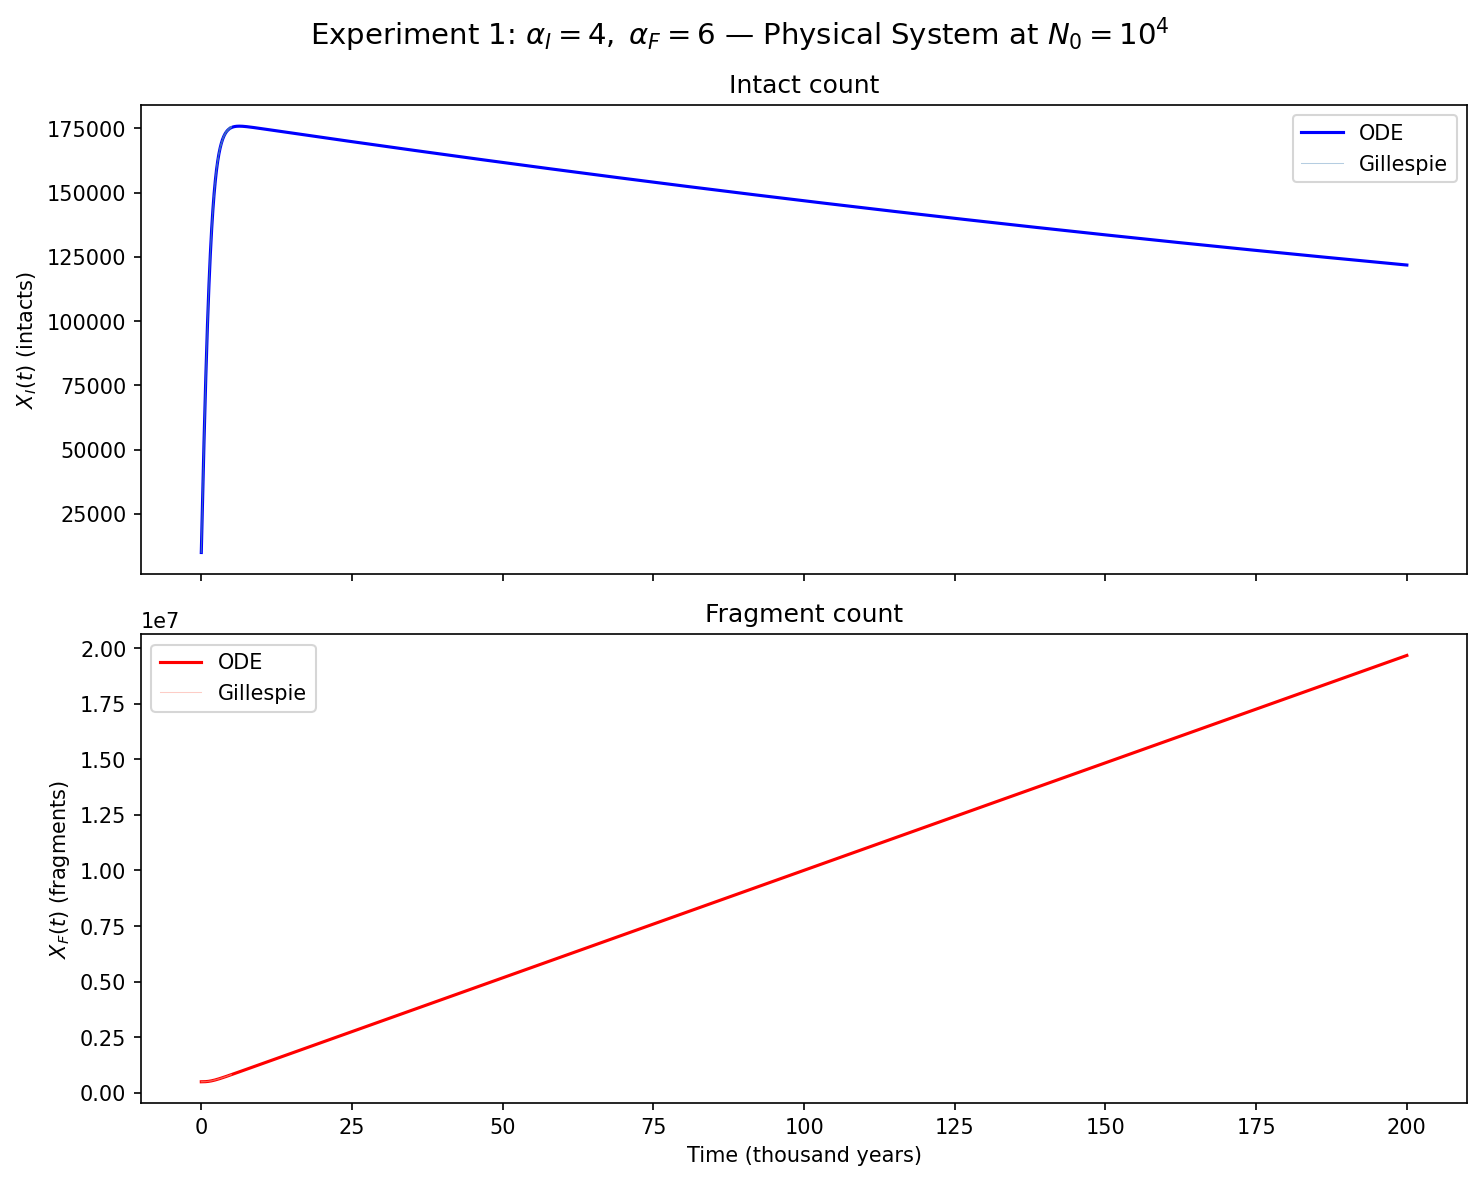
\includegraphics[width=0.85\textwidth]{figures/exp1_physical.png}
    \caption{Experiment~1: Physical system trajectories $(X_I(t), X_F(t))$ at $N_0 = 10^4$. Blue: ODE (deterministic fluid limit). Light traces: Gillespie SSA realizations.}
    \label{fig:exp1_physical}
\end{figure}

\begin{figure}[htbp]
    \centering
    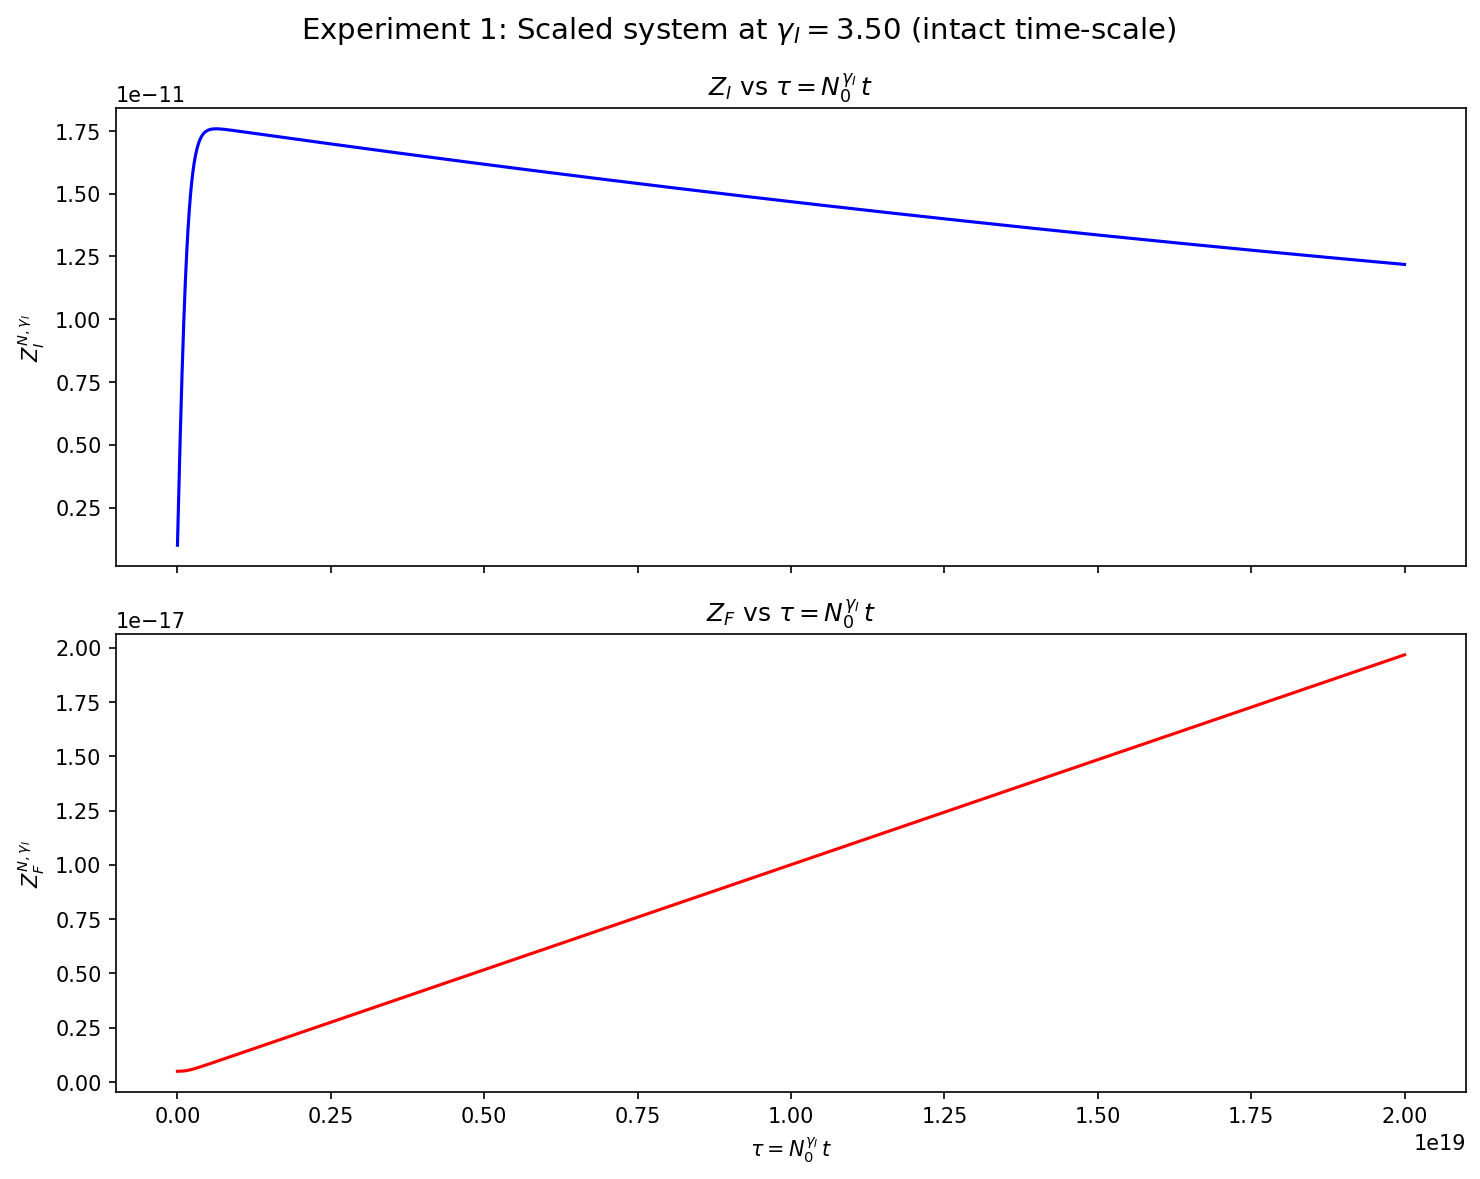
\includegraphics[width=0.85\textwidth]{figures/exp1_scaled_gammaI.png}
    \caption{Experiment~1: Scaled system $(Z_I^{N,\gamma_I}, Z_F^{N,\gamma_I})$ at the intact time-scale $\gamma_I = 3.5$.}
    \label{fig:exp1_gammaI}
\end{figure}

\begin{figure}[htbp]
    \centering
    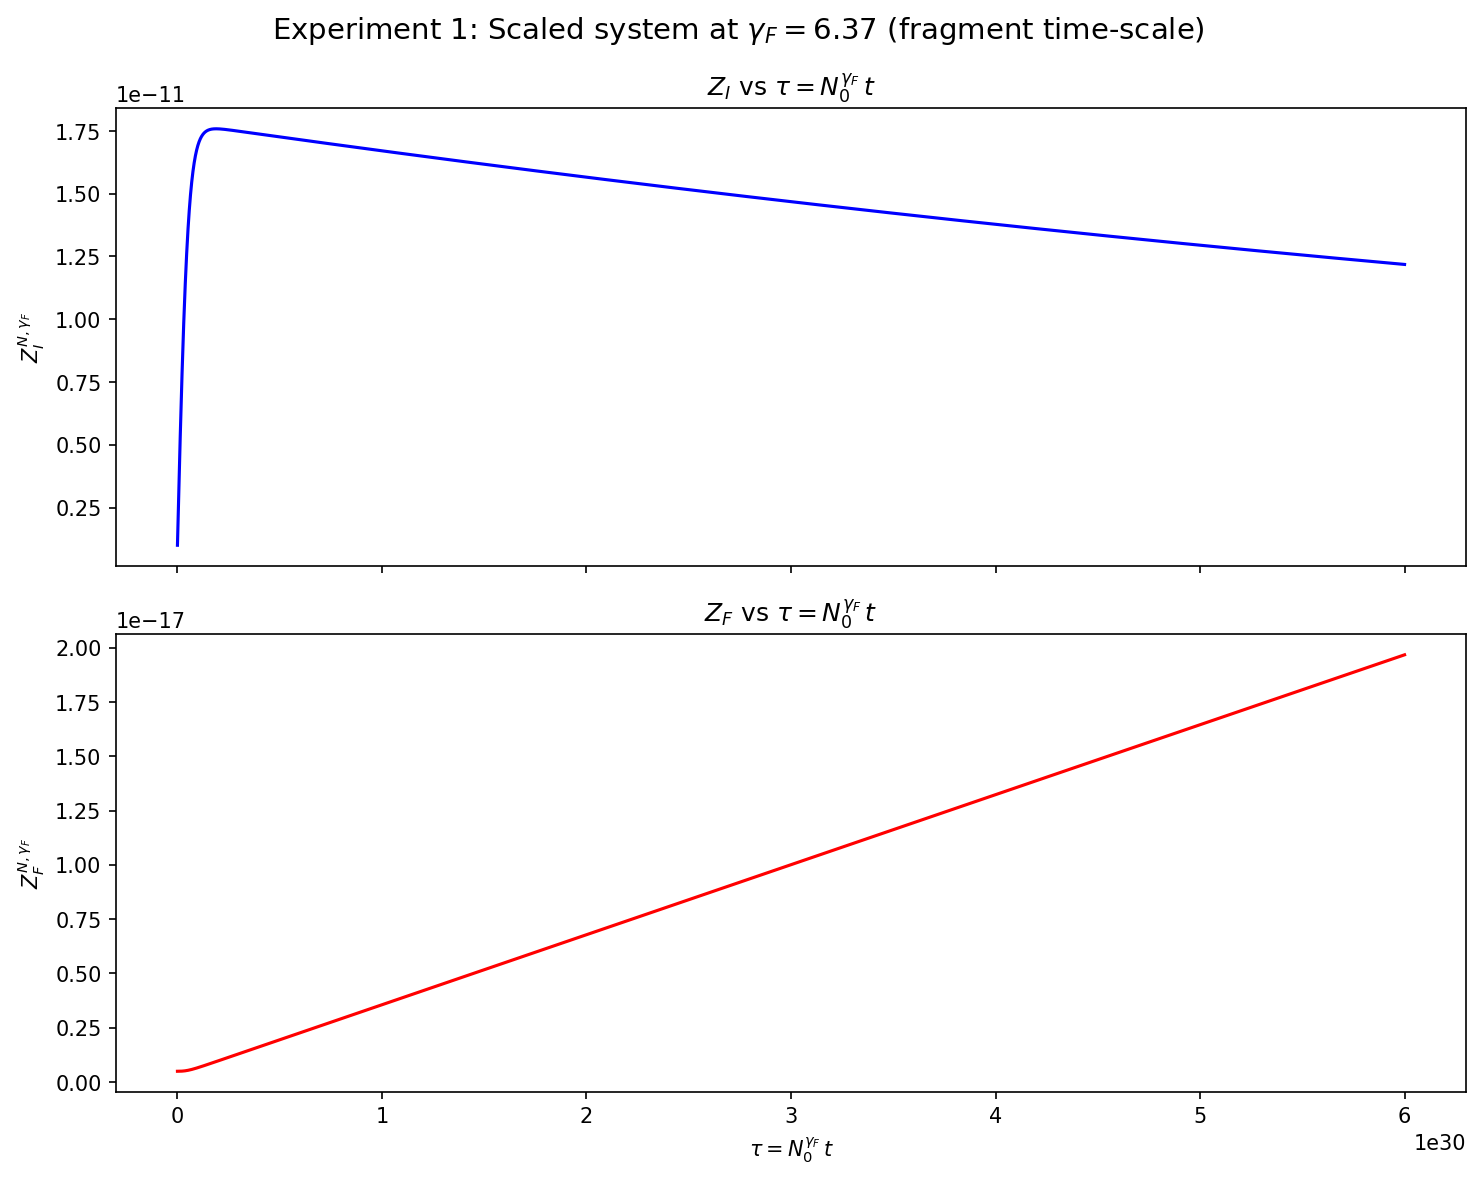
\includegraphics[width=0.85\textwidth]{figures/exp1_scaled_gammaF.png}
    \caption{Experiment~1: Scaled system $(Z_I^{N,\gamma_F}, Z_F^{N,\gamma_F})$ at the fragment time-scale $\gamma_F \approx 6.37$.}
    \label{fig:exp1_gammaF}
\end{figure}

\begin{figure}[htbp]
    \centering
    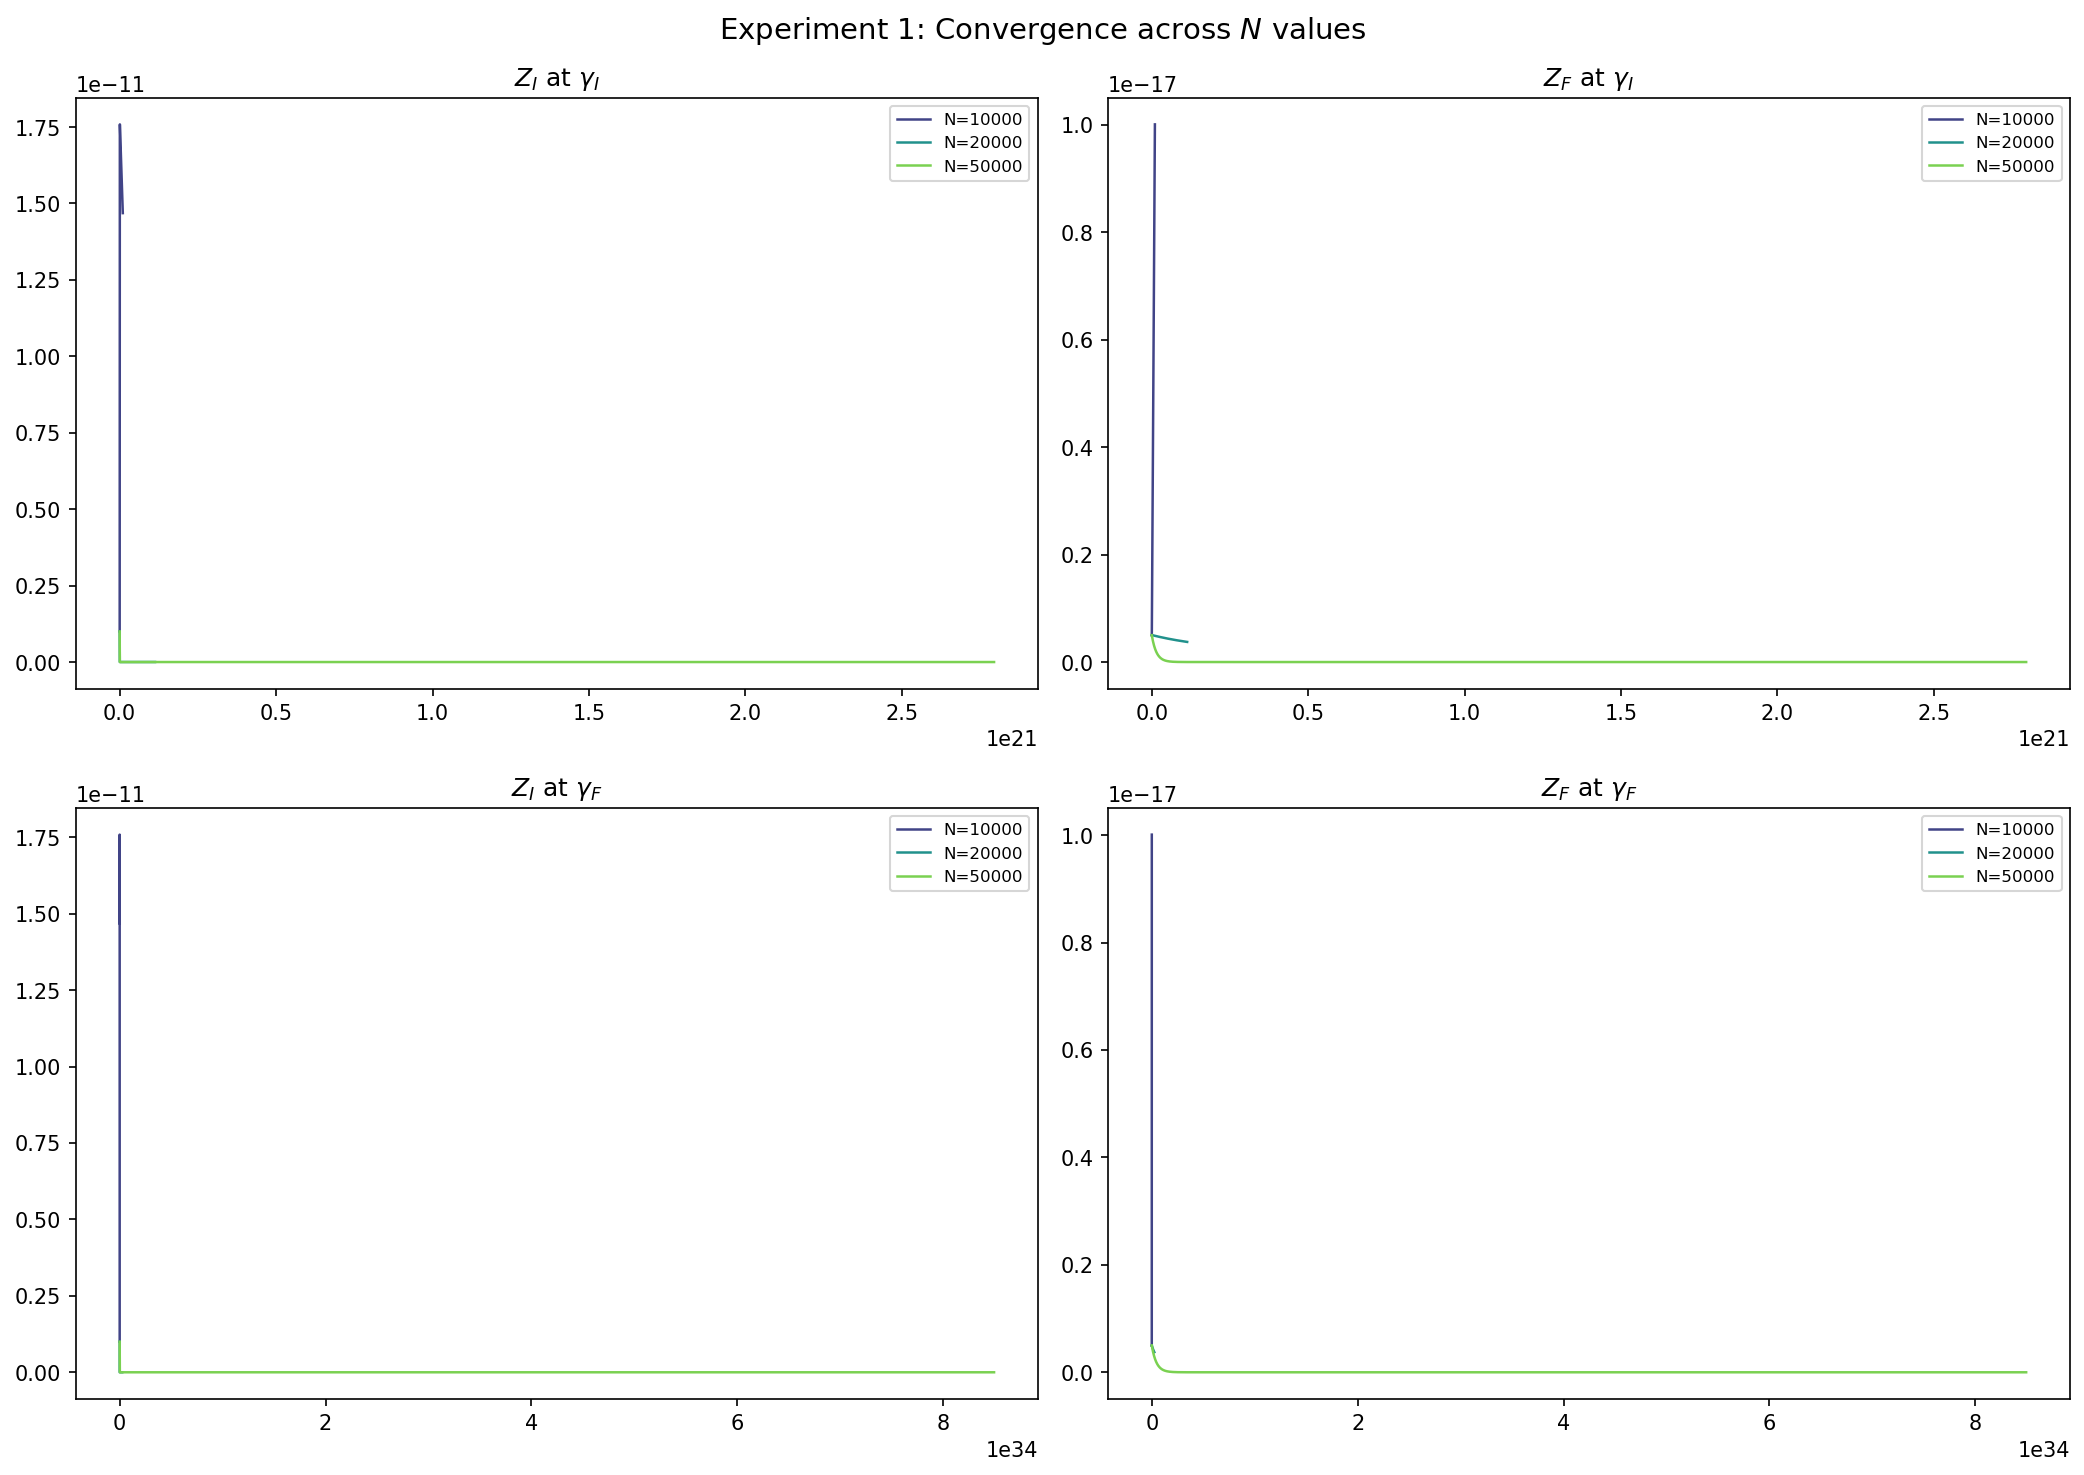
\includegraphics[width=0.85\textwidth]{figures/exp1_convergence.png}
    \caption{Experiment~1: Convergence of scaled trajectories across $N$ values. As $N$ increases, the scaled variables $Z_I, Z_F \to 0$, reflecting that $\alpha_I = 4$ and $\alpha_F = 6$ exceed the natural abundances of the reference system.}
    \label{fig:exp1_convergence}
\end{figure}

\subsection{Experiment 2}
Choose $\alpha_I = 0$ and $\alpha_F = \frac32$.
The time-scales are $\gamma_I = \alpha_I - \rho_1 = -0.5$ and $\gamma_F = \alpha_F - \rho_5 \approx 1.87$.
Note that $\gamma_I < 0$, which indicates that the balance condition $\alpha_I \geq \rho_1$ is not satisfied for this choice of $\alpha_I$.

Figure~\ref{fig:exp2_physical} shows the physical system trajectories.
Figures~\ref{fig:exp2_gammaI} and~\ref{fig:exp2_gammaF} show the scaled variables at the intact and fragment time-scales.
Figure~\ref{fig:exp2_convergence} shows the multi-$N$ convergence.
Figure~\ref{fig:exp2_kessler} shows the Kessler threshold: the critical intact count $X_I^{\mathrm{crit}} = \kappa_5/\kappa_3 = 3000$ above which fragments grow unboundedly.

\begin{figure}[htbp]
    \centering
    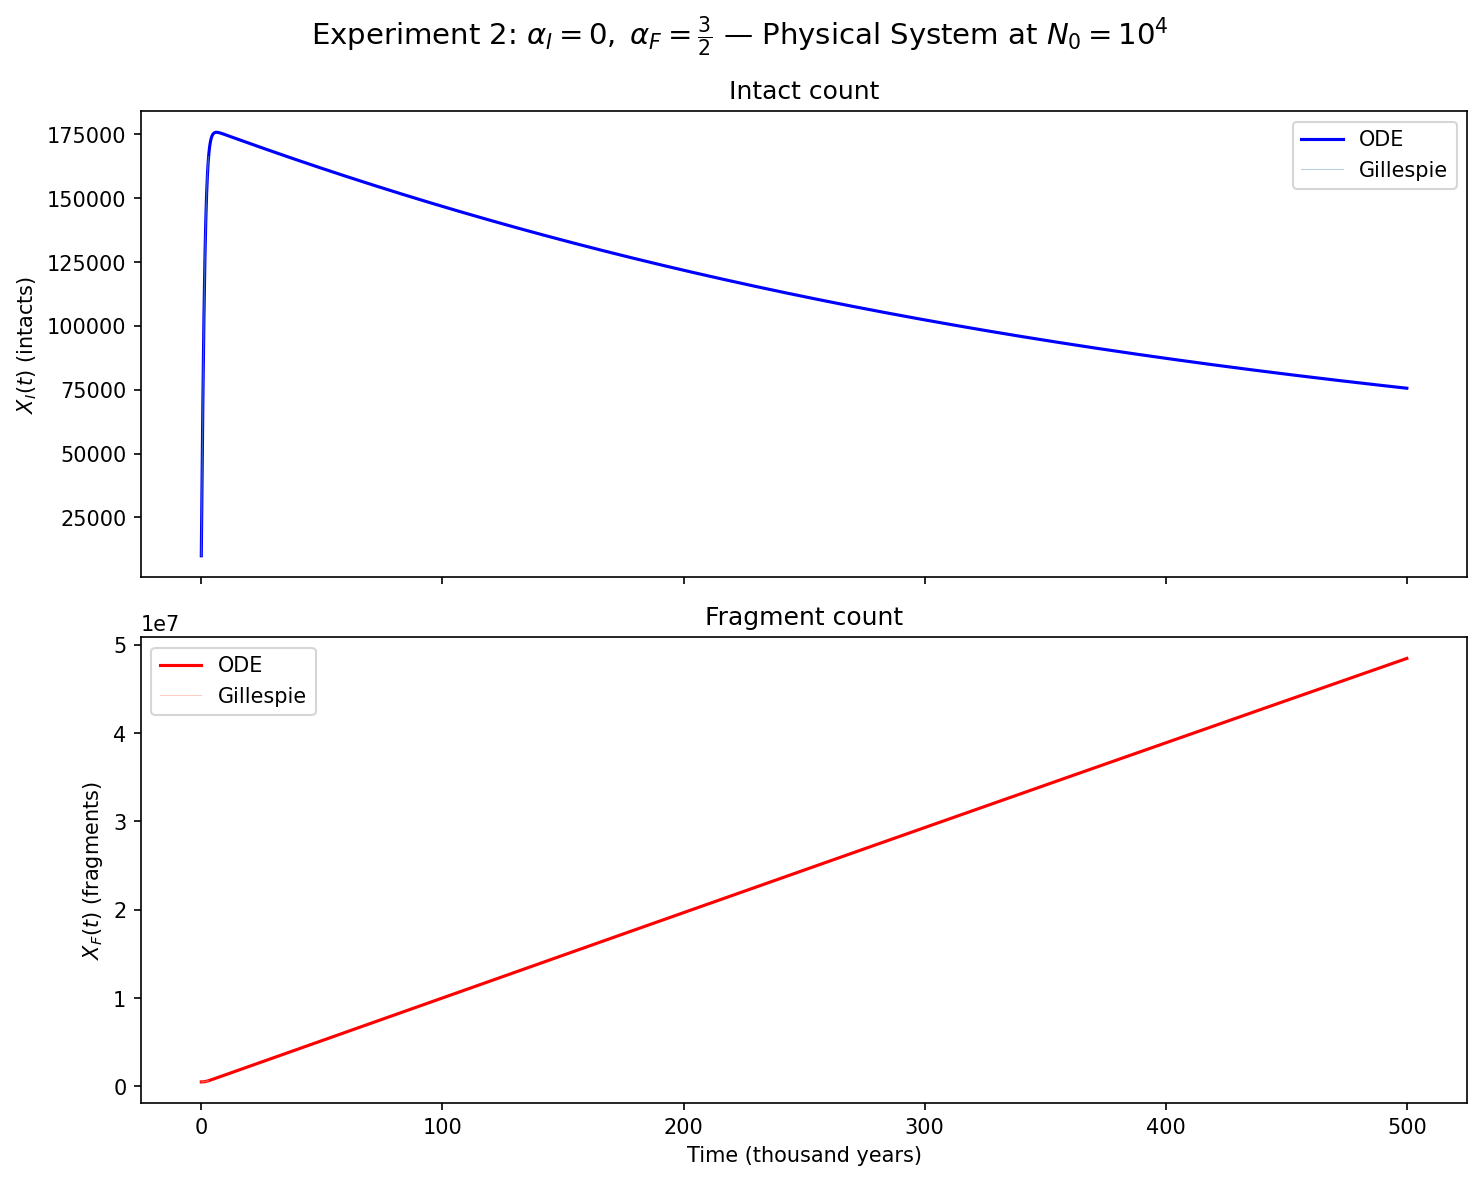
\includegraphics[width=0.85\textwidth]{figures/exp2_physical.png}
    \caption{Experiment~2: Physical system trajectories $(X_I(t), X_F(t))$ at $N_0 = 10^4$.}
    \label{fig:exp2_physical}
\end{figure}

\begin{figure}[htbp]
    \centering
    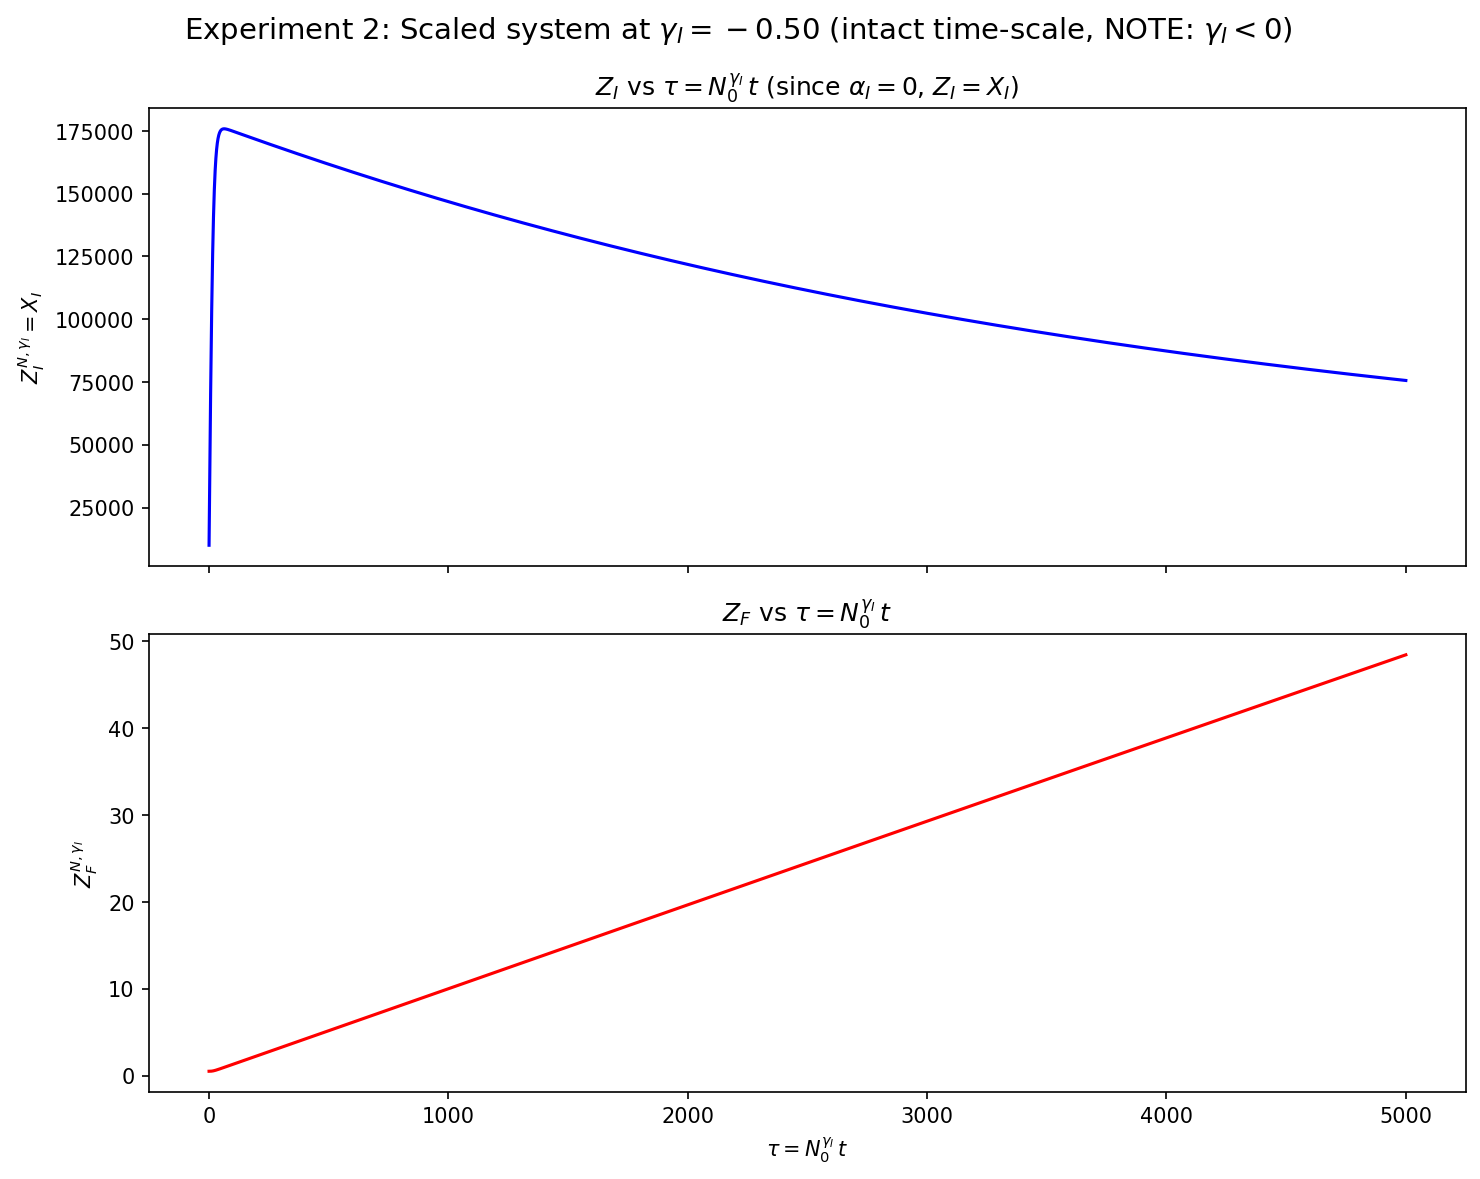
\includegraphics[width=0.85\textwidth]{figures/exp2_scaled_gammaI.png}
    \caption{Experiment~2: Scaled system at the intact time-scale $\gamma_I = -0.5$. Since $\alpha_I = 0$, $Z_I = X_I$.}
    \label{fig:exp2_gammaI}
\end{figure}

\begin{figure}[htbp]
    \centering
    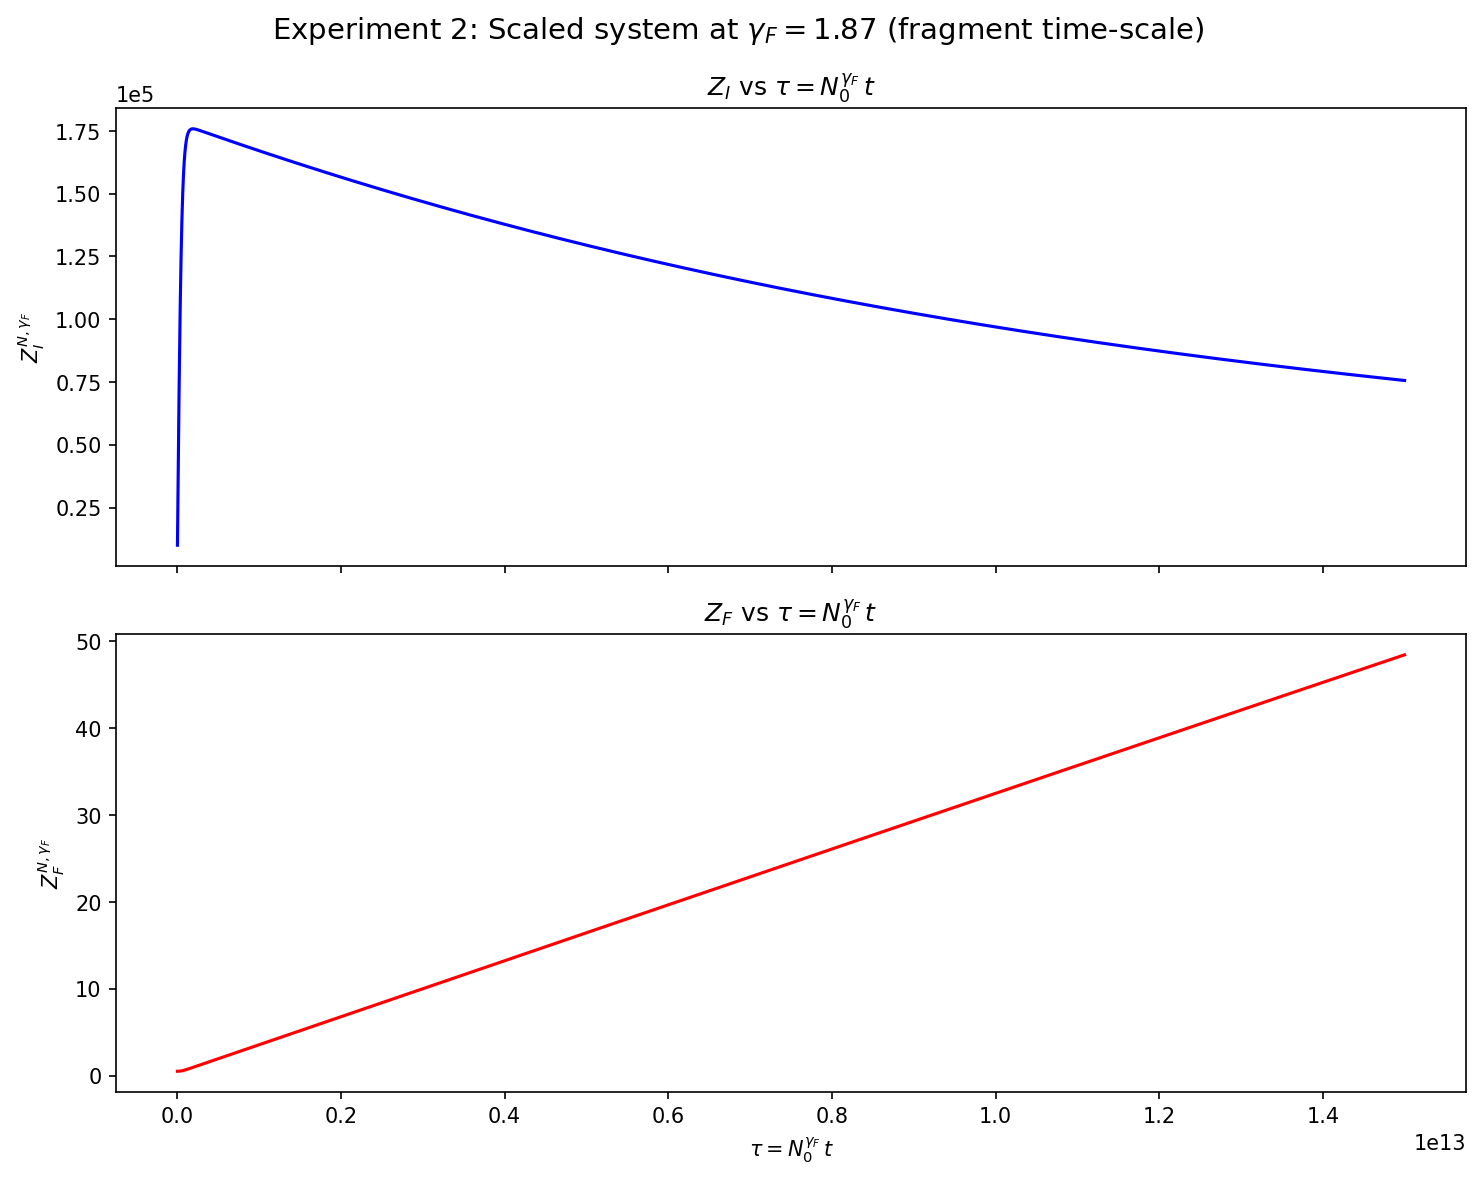
\includegraphics[width=0.85\textwidth]{figures/exp2_scaled_gammaF.png}
    \caption{Experiment~2: Scaled system at the fragment time-scale $\gamma_F \approx 1.87$.}
    \label{fig:exp2_gammaF}
\end{figure}

\begin{figure}[htbp]
    \centering
    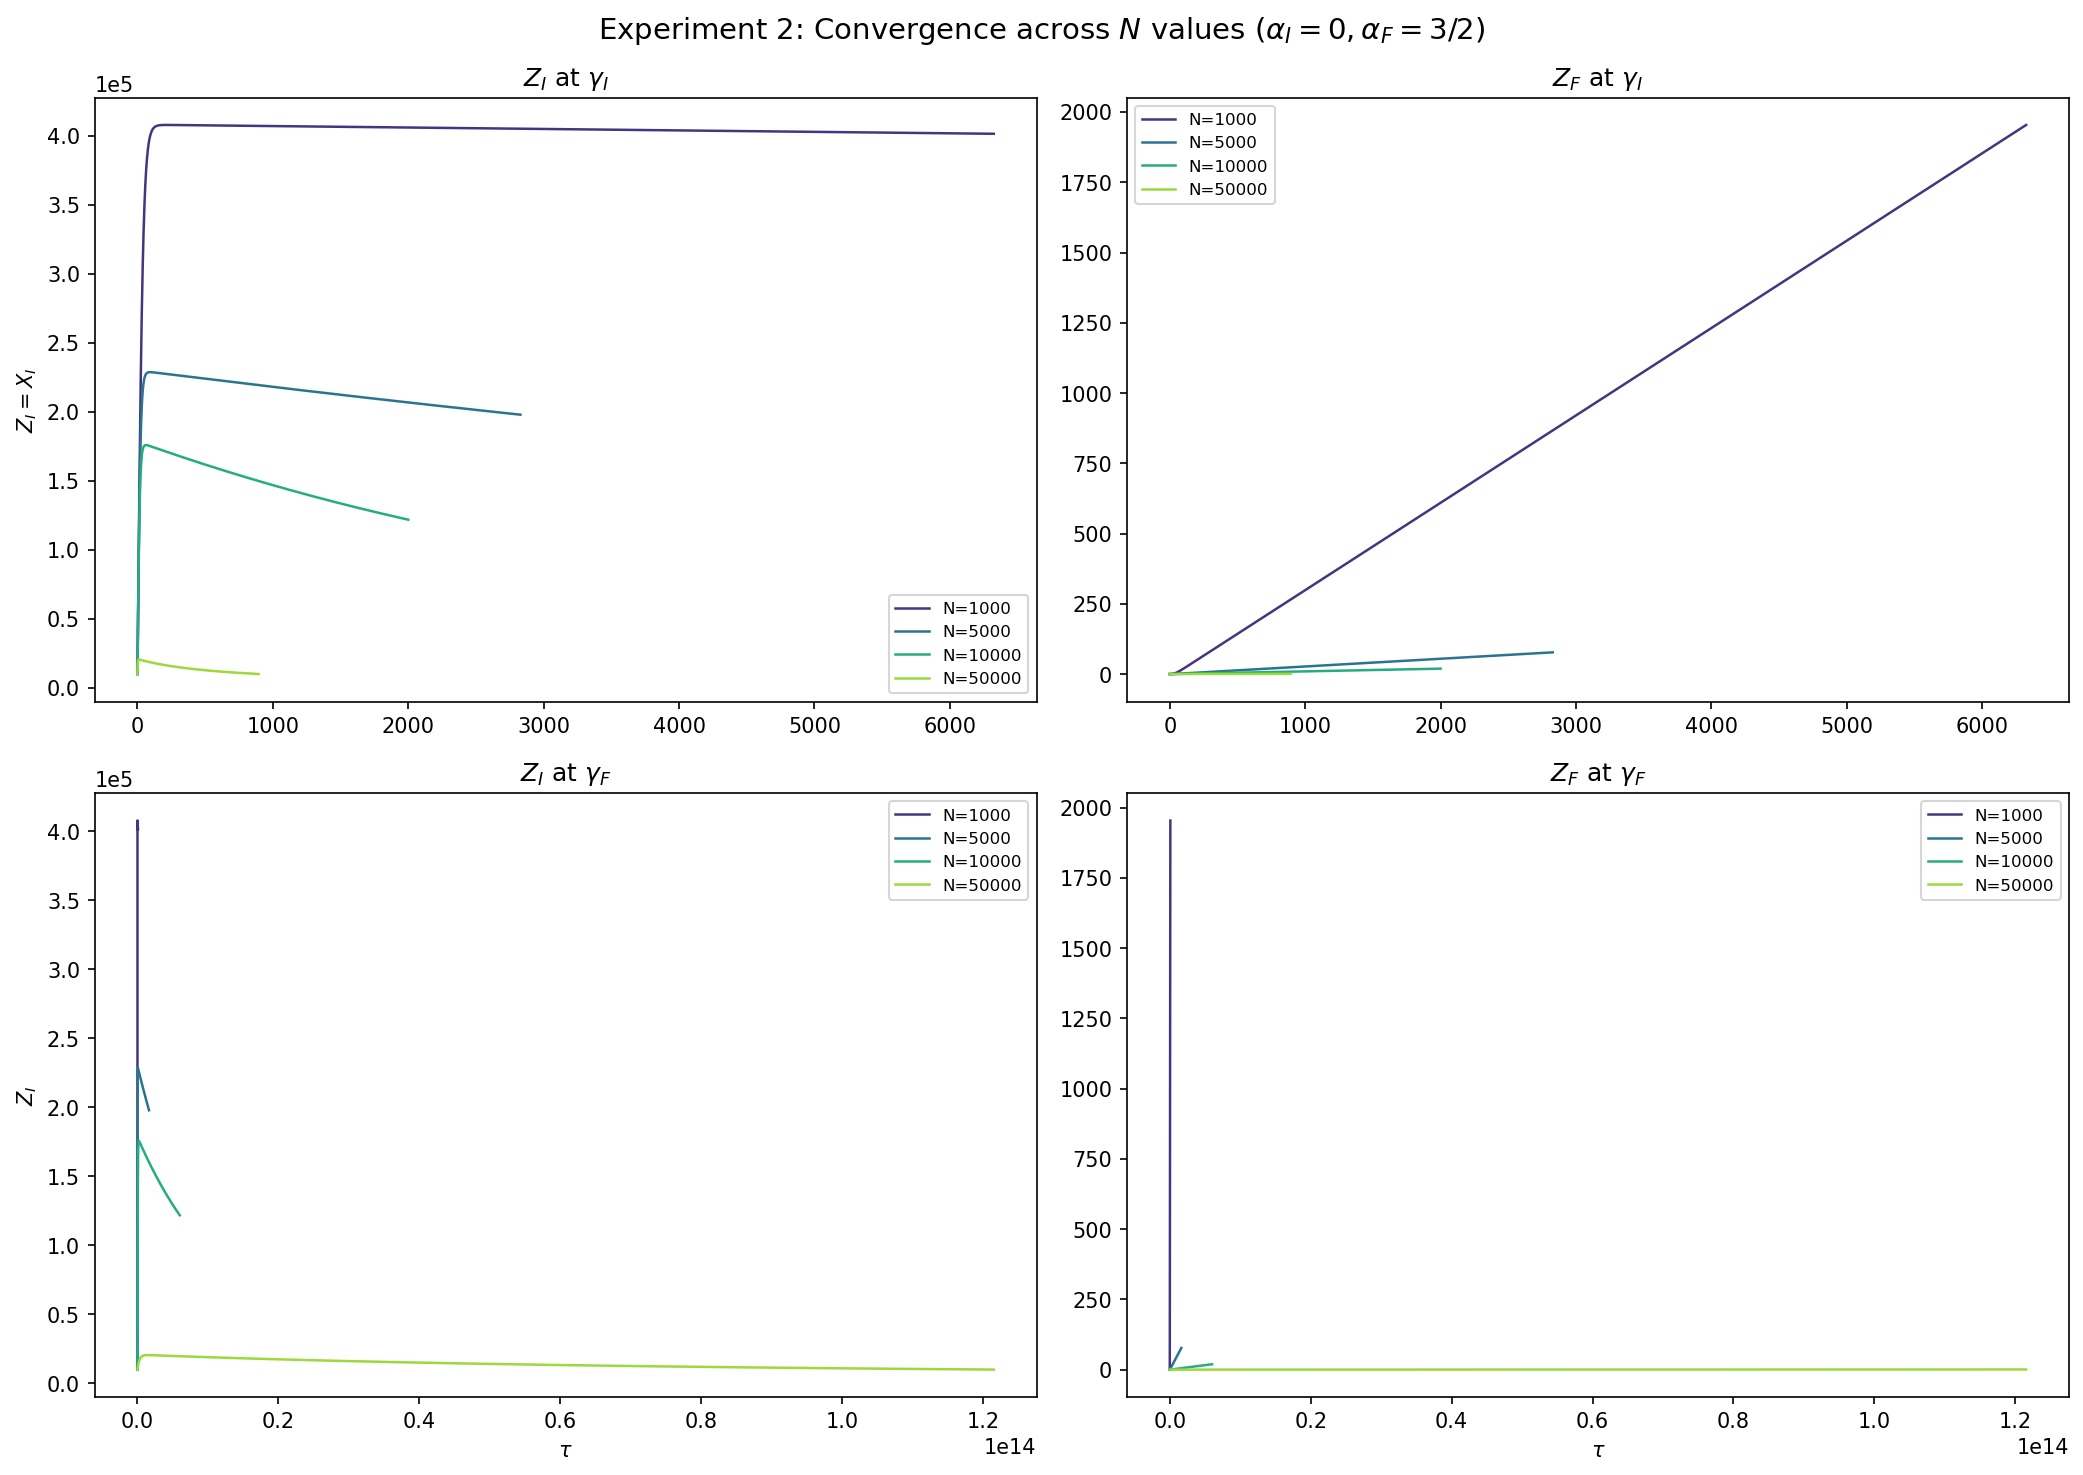
\includegraphics[width=0.85\textwidth]{figures/exp2_convergence.png}
    \caption{Experiment~2: Convergence of scaled trajectories across $N \in \{10^3, 5\times 10^3, 10^4, 5\times 10^4\}$.}
    \label{fig:exp2_convergence}
\end{figure}

\begin{figure}[htbp]
    \centering
    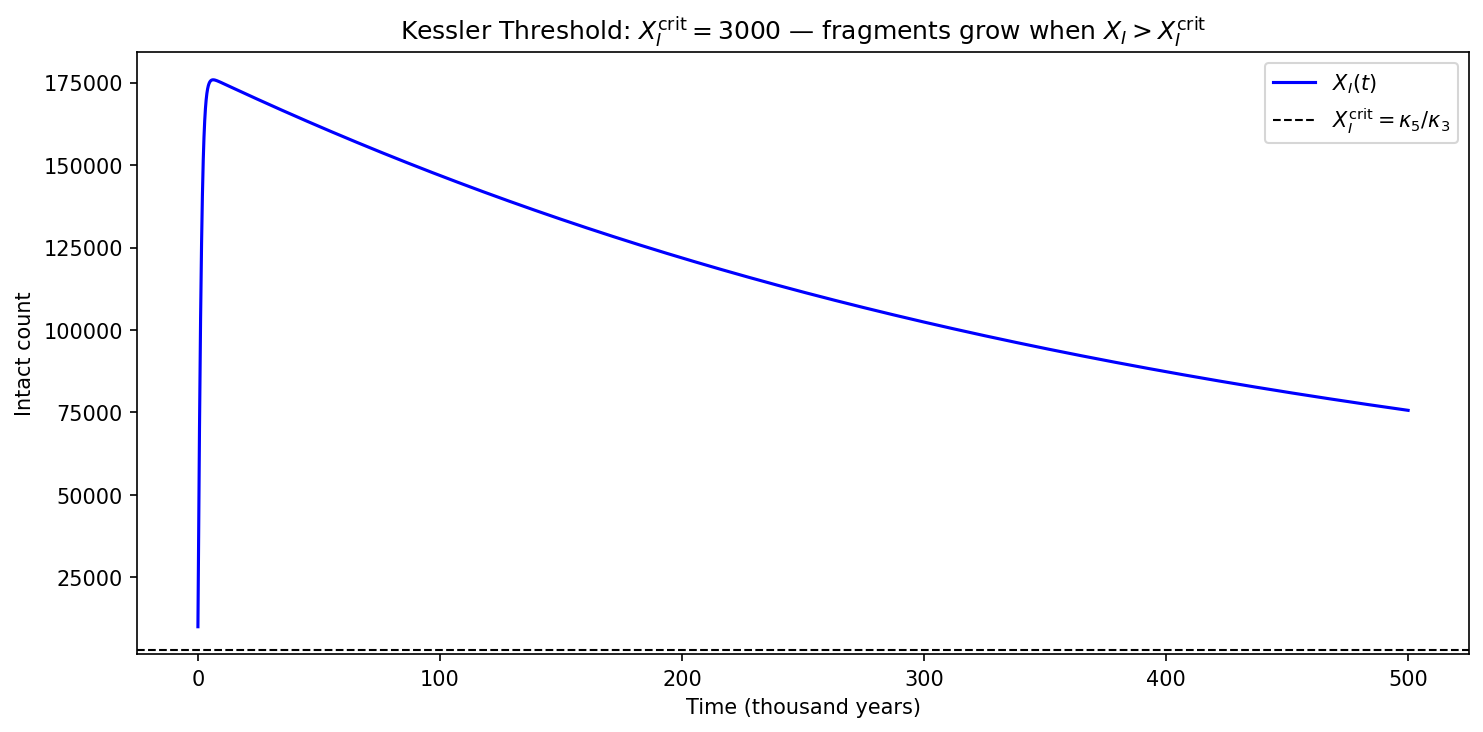
\includegraphics[width=0.85\textwidth]{figures/exp2_kessler.png}
    \caption{Kessler threshold: $X_I^{\mathrm{crit}} = \kappa_5/\kappa_3 = 3000$. Since $X_I(0) = 10^4 > X_I^{\mathrm{crit}}$, fragments grow throughout the simulation.}
    \label{fig:exp2_kessler}
\end{figure}

\end{document}
